
\chapter{Active contours : GVF Snakes}\label{ch:active-contours-:-gvf-snakes}
\chead{}
\lhead{\bfseries \chaptername {\,} \thechapter }
\cfoot{\bfseries \thepage}
\rhead{}
\rhead{\bfseries Active contours : GVF Snakes}

\section{Introduction}\label{sec:introduction-ch2}
Active contours take their origin from the elastic models but the
community grants itself to attribute them to theKass, Witkin and
Terzopoulosteam, \cite{2.1} who introduce snakes or minimizing curves. Snakes take
their name from their ability to deform like snakes. Since the publication of this
team, deformable models have become a very important subject for the image
processing community.\\
The active contour model is a sequential technique for image segmentation.
Given an approximation of the boundary of an object in an image, an active
contour model is used to find the actual boundary by deforming the initial
boundary to lock onto features of interest within this image. There are many
fields of use in both 2D and 3D, such as image segmentation, pattern
recognition, scene tracking, and simulation. In this chapter, we will first see
some definitions that will allow us to understand the principle of active
contours.

\section{Classic Active contours}\label{sec:classic-active-contours}

An active contour (snake) is formed by a list of moving and distributed points
on a two-dimensional curve.Which are typically initialized outside the object of
interest, the curve move under the influence of several forces that will pull it or
push it towards the object, the evolution of curve is done through an iterative
process that deforms the curve at each iteration up to its final position see figure(\ref{fig:figure1}).

\begin{figure}[h]
        \centering
        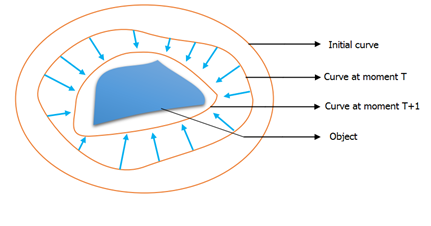
\includegraphics[width=10cm]{chapiter2/figures/Figure 01 the active contour (snake).png}
        \caption{The active contour (snake)}\label{fig:figure1}
\end{figure}
\vspace{1cm}

\hspace{-0.6cm}Snake introduced by Kass, Witkin and Terzopoulos \cite{2.1}, the idea started from
making the initial closed curve converge to the desired object by minimizing
the energy functional.The name "snake" is the reason for the appearance of
the parametric curve, which changes during the iterative process.\\
Snake is designed to vary its shape and position while tending to search
through the minimal energy state. Snake propagates through the domain of the
image to reduce the energy function and intends to dynamically move to the
local minimum. Snake is expressed by Eq(\ref{eq:eq01}). The parametric form of the curve
is exploited in the Snake model that has more advantages than utilizing implicit
and explicit curve forms.\\
\begin{equation}
        V(s, t) = (x (s, t), y (s, t))\label{eq:eq01}
\end{equation}
Where x and y are the coordinates of the two-dimensional curve, v is the spline parameter
in the range 0-1, s is linear parameter $\in$ [ 0,1], and t is time parameter $\in$ [ 0,$\infty$].\\
The forces in the snake include external forces as well as image forces that help in feature identification.When
the snake model moves around a closed curve, it moves with the influence of both internal and external energy
to keep the total energy minimum \cite{2.2}.\\
the energy is usually formed by internal forces and external forces are described in Eq(\ref{eq:eq02}).
\begin{equation}
        E_{snack} = E_{internal} + E_{external}.\label{eq:eq02}
\end{equation}

\hspace{-0.6cm}$E_{internal}$ tends to elastically hold the curve together (elasticity forces) and
to keep it  from bending too much (bending forces) and the external energy  pushes the snake line 
to the actual contours of the object in the image \cite{2.3}.

\subsection{Energy}\label{subsec:energy}
As we have already seen a snake is a parametric curve that move into a position where its energy is minimized.
Kass, Witkin and Terzopoulos \cite{2.1} have introduced the following energy functional for calculating the snake energy:
\begin{equation}
        \begin{aligned}
                E_{snake} & = \int_{0}^{1} E_{internal}(V(s)) + E_{external}(V(s)) ds \\
                          & = \int_{0}^{1} E_{internal}(V(s)) + E_{img}(V(s)) + E_{con}(V(s)) ds
        \end{aligned}
        \label{eq:eq03}
\end{equation}


\hspace{-0.6cm}The snake energy consist of three terms:\\
The first term $E_{internal}$ denotes the internal energy of the snake while the second term $E_{img}$ represents the image
forces, the last term $E_{con}$ gives rise to external constraint forces.
The sum of the image forces $E_{img}$ and the external constraint forces $E_{con}$ is also simply known as
the external snake forces denoted by $E_{external}$.

\subsubsection{Internal energy}
Internal energy it does not depend on the image or the shape, it depends only
on the points of the contour, so it is related to the Snake. The internal energy
of the snake is the component of the behavior function that describe the
physical properties of our contour like smoothness or continuity and curvature
It usually consists of two Terms:
\begin{equation}
        E_{internal} = \frac{1}{2}(\alpha(s)\| V_s (S) \| ^2 + \beta(s)\mid\mid V_{ss} (S) \mid\mid^2)\label{eq:equ04}
\end{equation}

\hspace{-0.6cm}The first-order term $\| V_s (S) \|^2$  measures the continuity (elasticity) or
smoothness which it's a function of the first derivative of our contour and it is
controlled by the coefficients $\alpha$, The elasticity force has the effect of making
the curve shrink even when it is not deformed. Thus, the shrinking effect allows
us to place the snake around the object we wish to find the contour of, and
then be fairly certain that it will come in contact with the image energy of the
object. However, it might be necessary to adjust the parameter $\alpha$ to prevent
the elasticity force from overcoming the image energy completely, as this
would result in the snake disregarding the image energy and shrinking into a
single point \cite{2.4}.\\
The second-order term represents the curvature force, which is the second
derivative of the parametric curve that used to measure how much the snake
curves at a point. Usually, the curvature is given by the second derivative of the
curve with regards to the arc length which controlled by the parameter $\beta$\cite{2.4}. It helps to prevent the contour from
containing isolated points that would not be consistent with the shape.

\subsubsection{Image energy}
Image energy take into account the characteristics of processed images ,which
pulls the active contour towards features in the image and can be defined as
suggested by Kass et al \cite{2.1} using the image intensity gradient:

\begin{equation}
        E_{image} (V(s)) = -\mid \nabla I(x,y) \mid^2\label{eq:eq05}
\end{equation}

\hspace{-0.6cm}Where I is the image function and $\nabla$ Laplacian operator.\\
The snake will try to position itself in areas of low energy, often the snake
should be attracted toward different image features as edges in the image.
Because, the image has noise that obstructs the snake moving, the image can
be smoothing to reduce the noise, the image can be convolved with a Gaussian
kernel before computing the gradients that increase the capture range of the snake, this gives the following
image energy term:
\begin{equation}
        E_{image} (V(s)) = -\mid \nabla [G_{\sigma}(x,y) * I(x,y)] \mid^2\label{eq:eq06}
\end{equation}

\hspace{-0.6cm}Where $G_\sigma(x, y)$ is a two dimensional Gaussian with standard deviation $\sigma$. When
strong edges in the image are blurred by the Gaussian the corresponding
gradient is also smoothed which results in the snake coming under the
influence of the gradient forces from a greater distance, hereby increasing the
capture range of the snake.The negative sign reverses the energy so that sharp
edges are mapped to areas of low energy\cite{2.4}.

\subsubsection{Context energy}
Context energy expresses some additional constraints that may be imposed by
the user according to the Snake he wants to obtain, we can example impose a
minimum or maximum distance between two consecutive points of the active
contour.\\
Among the energies of context one finds, the energy of balloon which
introduced by L. D. Cohen and I. Cohen \cite{2.5},This model is based on an additional
inflation force applied to give stable results. A snake, which is not close the
contours is not attracted by them. The curve behaves like a balloon, which is
inflated. The balloon force is calculated as follow:
\begin{equation}
        F = K_1n(s) - K \frac{\nabla P}{\| \nabla P \|}\label{eq:eq07}
\end{equation}

\hspace{-0.6cm}Where n(s) is the normal unitary vector to the curve at point u(s) and $k_1$ is the
amplitude of this force. The sign of $k_1$ or the orientation of the curve has the
effect of deflation or the inflation of the snake \cite{2.5} (when $k_1$ is positive it will
concentrate the snake, while a negative coefficient will make the snake
expansive).
\section{Energy Minimization}\label{sec:energy-minimization}

Several methods have been proposed to solve the problem of minimization of
the functional energies $E_{snake}$ there are three main method:

\subsection{The variation approach}\label{subsec:the-variation-approach}
Using only the first two energy types of equation Eq (\ref{eq:eq03}) which are
control (smoothing + stiffness) and energy of the gradient, we end up with
theformulation of active contours introduced by Kass, Witkin and
Terzopoulos \cite{2.1}.\\
Minimizing the energy functional of Eq (\ref{eq:eq03}) gives rise of the following two
independent Euler equations:
\begin{equation}
        \begin{matrix}
                - \alpha x_{ss} + \beta x_{ssss} + \frac{\sigma E_{ext}}{\sigma x} = 0 \\
                - \alpha y_{ss} + \beta y_{ssss} + \frac{\sigma E_{ext}}{\sigma y} = 0
        \end{matrix}
        \label{eq:eq08}
\end{equation}

\hspace{-0.6cm}To solve numerically, the Euler equations with $f_x =\frac{\sigma E_{ext}}{\sigma_{x_i}}$ 
and $f_y =\frac{\sigma E_{ext}}{\sigma_{y_i}}$ are discretized, yielding :\\
\begin{equation}
        \begin{aligned}
                \alpha_i & (v_i - v_{i-1}) - \alpha_{i+1} (v_{i+1} - v_i) \\
                 & + \beta_{i-1}(v_{i-2} - 2v_i + v_i ) \\
                 & - 2 \beta_i (v_{i-1} -2v_i + v_{i+1}) \\
                 & + \beta_{i+1} (v_i -2v_{i+1} + v_{i+2}) + (f_x(i),f_y(i)) = 0.
        \end{aligned}
        \label{eq:eq09}
\end{equation}
The above Euler equations can be written in matrix forms, one for x and
another for y, yields:
\begin{equation}
        \begin{matrix}
                Ax + + f_x(x,y) = 0 \\
                Ay + + f_y(x,y) = 0.
        \end{matrix}
        \label{eq:eq10}
\end{equation}

\hspace{-0.6cm}Now it's can be solve for position vectors iteratively :
\begin{equation}
        \begin{matrix}
                x_t = (A + \gamma I)^{-1} (\gamma x_{t-1} - f_x(x_{t-1}, y_{t-1})) \\
                y_t = (A + \gamma I)^{-1} (\gamma y_{t-1} - f_y(x_{t-1}, y_{t-1}))
        \end{matrix}
        \label{eq:eq11}
\end{equation}

\hspace{-0.6cm}As characteristics of the formulation, if a contour is not subjected to any
external forces, it will vanishto a line or a point, and furthermore, if it is not
placedclose to image boundaries, it will not get attracted.\\
In summary, although the computational requirementsof the variational
approach is linear, dynamic programming has important features, making the
new formulation attractive \cite{2.6}.
\subsection{Discrete dynamic programming}\label{subsec:discrete-dynamic-programming}
Dynamic programming is a classic method of solving optimization problems.Its
application to active contours can be an interesting alternative to variational
calculation.\\
By Discretizing the integral in The Eq(\ref{eq:eq03}) can be written as follow\cite{2.6}:

\begin{equation}
        E * E_{tot} = \sum_{i = 0}^{n} E_{int} (v_i) + E_{ext} (v_i).
        \label{eq:eq12}
\end{equation}

\hspace{-0.6cm}In order to use dynamic programming, the minimization of Eq (\ref{eq:eq12}) can be
viewed as a discrete multistage decision process Starting from the initial point
on the contour, we can treat the minimization problem as one that at each of a
finite set of stages ($i_{0},i_{1},\ldots, i_{n-1}$) It is possible to express $E_{tot}$:

\begin{equation}
        E(v_1,v_2,\ldots,v_n) = E_1(v_1,v_2) + E_2(v_2,v_3) + \cdots + E_{n-1}(v_{n-1},v_{n}).
        \label{eq:eq13}
\end{equation}

\hspace{-0.6cm}But this come back to a problem of optimization of a numerical function a
several variables. \\
The variables will be the positions of the different points of
the snake where each variable is allowed to only take on m possible values. The
standard formulation in recurrent form of programming dynamic can be
written:\\

\begin{equation}
        S_i(v_{i+1},v_i) = min S_{i-1}(v_i,v_{i-1}) + \alpha (\mid v_i - v_{i-1} \mid)^2 + \beta \mid v_{i+1} - 2v_i + v_{i-1} \mid ^2 + E_{ext}(v_i).
        \label{eq:eq14}
\end{equation}

\hspace{-0.6cm}Each iteration gives an optimal contour. The convergence of the energy is
guaranteed but it's has a high complexity (The time complexity for the
algorithm increases to O($nm^3$),(where n is the length of the contour and mis
the number of possible choices at each stage).

\subsection{Greedy Method}\label{subsec:greedy-method}
The greedy method is a discrete nature technique introduced by[7], which used
to simplify the minimization of snake energy.The primary characteristic of the
greedy snake is that it computes the movement of each snake point by looking
at the neighborhood of pixels around the snake point and then moving the
snake point to the position in the neighborhood that minimizes the energy
term. The energy functional for the contour defined as follows:
\begin{equation}
        \begin{aligned}
                E_{snake} & = \int_{0}^{1} E_{snake}(V(s)) ds \\
                & = \int_{0}^{1} E_{internal}(V(s)) + E_{external}(V(s)) ds \\
                & = \int_{0}^{1} E_{internal}(V(s)) + E_{img}(V(s)) ds
        \end{aligned}
        \label{eq:eq15}
\end{equation}

\hspace{-0.6cm}The image energy of the greedy snake is calculated as:
\begin{equation}
        E_{img}(V(s)) = \mid \nabla [G \sigma(x,y) * I(x,y)] \mid^2
        \label{eq:eq16}
\end{equation}
Which is almost the same energy term as in the Kass et al,except that there is
missing a minus in front of the term.Therefore, the image energy in the
neighborhood of the snake control point V (si) has to be normalized in a
manner that assigns large negative values to pixels with high gradient values,
while assigning lower negative values to pixels with a lower gradient value. The
gradient magnitudes are all in the interval [0; 255]. The normalization of the
neighborhood is calculated as:
\begin{equation}
        Location(x,y) = \frac{min-mag(x,y)}{max - min}
        \label{eq:eq17}
\end{equation}

\hspace{-0.6cm}Where min is the minimum gradient and max the maximum value in the
neighborhood, and mag(x, y) the gradient magnitude of the actual point \cite{2.7},this
normalization sets the highest gradient magnitude in the neighborhood to -1
and the lowest to 0. For example, whenall the gradient magnitude values are in
the interval [46, 49] then the normalized values would be 0, -0.33, -0.66 and -1.\\
The internal energy of the snake is divided in two terms $E_{ela}$ and $E_{cur}$ .\\
The greedy used a different way for calculating the elasticity term. Thus,
reducing the shrinking effect and making sure that the snake control points
does not bunch up in places with high image energy. The elasticity term in the
greedy is calculated in the neighborhood of each snake control point as:
\begin{equation}
        \bar{d} - \| v(s_i) - v(s_{i-1}) \| = \overline{d} - \sqrt{(x(s_i) - x(s_i) - 1)^2 +(y(s_i) - y(s_i) - 1)^2 }
        \label{eq:eq18}
\end{equation}

\hspace{-0.6cm}Where $\bar{d}$ is the average distance between all points in the snake. After term has
been calculated for each pixel in the neighborhood of a snake control point, the
points which having a distance near the average will have the minimum
value \cite{2.7}, so the minimum energy will be achieved when $\bar{d} - \| v(s_{i} - v(s_{i-1}) \| = 0$.\\
The neighborhood is normalized as all the values are divided by the largest
value in the neighborhood giving values between [0, 1], at the end of each
iteration a new value of $\bar{d}$ is computed \cite{2.7}. \\
The second term of internal energy, which represent the curvature force,In
Williams and M. Shah \cite{2.7} evaluate a set of different ways of calculating the
curvature term for a d discrete parametric curve whichcalculated in the
neighborhood of each snake control point as:
\begin{equation}
        \begin{aligned}
                E_{curv} & = | \vec{u}_i - \vec{u}_{i+1} |^2 \\
                & = | (p_{i-1} - p_i) - (p_i - p_{i+1}) | ^2 \\
                & = | p_{i-1} - 2p_i + p_{i+1} | ^ 2
        \end{aligned}
        \label{eq:eq19}
\end{equation}

\hspace{-0.6cm}Once the curvature has been calculated for each point in the neighborhood of
the current snake control point the values are normalized by dividing
with the largest value. So we ends up with all the curvature values being in
the range between [0, 1] as with the image and elasticity energy.\\
Finding a suitable value for the parameter $\alpha$ and $\beta$ is very important in the
greedy method, because its determine the extent to which the contour is
allowed to stretch or bend at all point. The relative sizes of $\alpha$ and $\beta$ can be
chosen to control the influence of the corresponding constraints (elasticity and
curvature)\cite{2.7} ,so choosing value of $\alpha$ and $\beta$ are making effect of snake
behavior see figure(\ref{fig:figure2}).

\begin{figure}[ht]
        \centering
        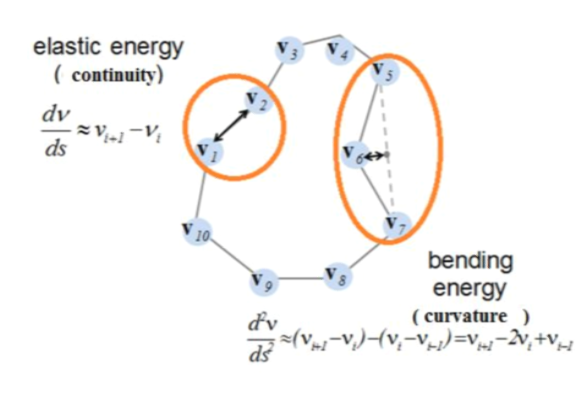
\includegraphics[width=10cm]{chapiter2/figures/Figure-02.png}
        \caption{Elastic and curvature energy in greedy}
        \label{fig:figure2}
\end{figure}
\vspace{4cm}

\hspace{-0.6cm}In the previous sections, we have explained how the energy of each term is
calculated for the greedy method. In this part, we will describe the actual
algorithm for how the points are moved.

\subsubsection{Greedy algorithm}
In the previous sections, we have explained how the energy of each term is
calculated for the greedy method. In this part, we will describe the actual
algorithm for how the points are moved.\\
For each point/pixel in the neighborhood of a snake control point, the three
energy terms are calculated. Then the algorithm sums the energy terms to get
the total energy:
\begin{equation}
        E_{comb}(x,y) = \alpha E_{ela}(x,y) + \beta E_{curv}(x,y) + \gamma E_{img}(x,y)
        \label{eq:eq20}
\end{equation}

\hspace{-0.6cm}Where $E_{ela}(x,y)$ is the elasticity energy, $E_{curv}(x,y)$ is the curvature energy and
$E_{img}(x,y)$ is the image energy and (x, y) are the indices to the points in the neighborhood.\\
Once the total energy has been calculated for each neighborhood, the greedy
algorithm moves the snake control point to the position that has the minimum
energy as it has shown in Figure(\ref{fig:figure3}), the values in the squares represent the
value of total energy. Also pictured is the snake control point v ($s_i$) and the
point before and after it.
\vspace{2cm}
\begin{figure}[ht]
        \centering
        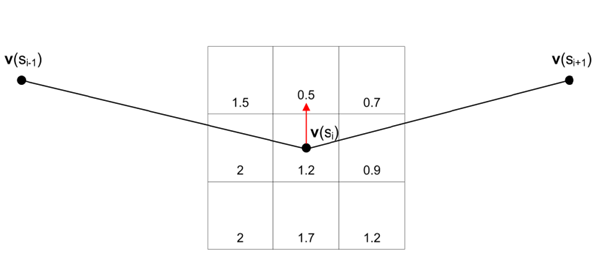
\includegraphics[width=10cm]{chapiter2/figures/Figure 3 The energy function is computed at vi and each of its eight.png}
        \caption{The energy function is computed at vi and each of its eight
        neighbors. The point before and after it on the contour are used in
        computing the continuity constraints. The location having the smallest
        value is chosen as the new position of $v(s_i)$ \cite{2.7}.}
        \label{fig:figure3}
\end{figure}

\hspace{-0.6cm}The red arrow shows to which point in the neighborhood the snake control
point will move.After all the control points along the snake have been moved
to a new position a new value of $\bar{d}$ is computed.
Algorithm(\ref{alg:algo-greedy}) demonstrates how the algorithm works.


\begin{algorithm}
        \SetKwData{Left}{left}\SetKwData{This}{this}\SetKwData{Up}{up}
        \SetKwFunction{Union}{Union}\SetKwFunction{FindCompress}{FindCompress}
        \SetKwInOut{Input}{input}\SetKwInOut{Output}{output}
%        \Input{A bitmap $Im$ of size $w\times l$}
%        \Output{A partition of the bitmap}
        \BlankLine
        \Repeat{$Pts_{moved} > threshold$}{
                \For{$i = 1$ \KwTo $n$}{
                        $E_{min} = infinity $ \;
                        \For{$j = 1$ \KwTo $m$}{
                                $E(j) = \alpha(i) E_{ela}(j) + \beta(i)E_{curv}(j) + E_{img}(j) $ \;
                                \If{$E(j) < E_{min}$}{
                                        $E_{min} = E(j)$ \;
                                        $j_{min} = j $ \;

                                        Move pint $v(i)$ to location $j_{min}$ \;
                                }
                                \If{$j_{min}$ is not the current location}{
                                        $Pts_{moved} ++$ \;
                                }
                        }
                }
        }
                \caption{greedy Algorithm}\label{alg:algo-greedy}
\end{algorithm}

%\fbox{%
%
%\parbox{\textwidth}{
%
%
%do  \color{blue}{ ”Main loop that moves the snake points to new locations”}\\ \color{black}
%for i = 1 to n \color{blue}“The first and last point in the snake are the same”\\\color{black}
%Emin = infinity\\
%for j = 1 to m \color{blue}“ m is the neighborhood size”\\ \color{black}
%E(j) = alpha(i) Eela(j) + beta(i) Ecurv(j) + Eimg(j)\\
%if E(j) < Emin then \color{blue} “Find location with min energy”\\ \color{black}
%Emin = E(j)\\
%jmin = j\\
%Move point v(i) to location jmin\\
%if jmin is not the current location then Ptsmoved++\\
%while Ptsmoved > threshold \color{blue}"Stop if only few points have moved "\\ \color{black}
%
%}
%}

\hspace{-0.6cm}The final step in the iteration of the greedy algorithm consists of checking
whether the number of points moved in the iteration is under the threshold
see algorithm(\ref{alg:algo-greedy}).\\
Threshold is used as a stopping criterion when the snake reach a
minimum energy, which mean most of the points have stopped
moving.
%
\section{Limit of active contour}\label{sec:Limit-of-active-contour}

The classical snakes have three main disadvantages, First, the active
contours have difficulties progressing into boundary concavities. The
second problem is that the initial contour must in general, be close to
the true boundary or else it will predict an incorrect result. Thirdly,
active contours need considerable processing time.\\
Convergence to concave regions is an issue, because the contour is often left
split across boundary concavities, as its shown figure (\ref{fig:figure4}) line drawing of a U-
shaped object having a concave region, which is obvious in figure (\ref{fig:figure4}) that the
snake fails to converge to the boundary concavity \cite{2.8}.\\
Initialization is a problem because the capture range of the traditional potential
force is generally small.The capture range can be increased by using a larger
$\sigma$,but this blurs and distorts the edges \cite{2.8}.
\begin{figure}[ht]
        \centering
        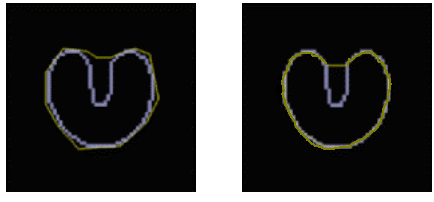
\includegraphics[width=10cm]{chapiter2/figures/Figure 5 the snake cannot move into the concave boundary region.png}
        \caption{The snake cannot move into the concave boundary region}
        \label{fig:figure4}
\end{figure}

\hspace{-0.6cm}The classic active contour also so sensitive the choice of the weights to be
assigned to each energy (the values of coefficients $\alpha, \beta, \gamma$); this is all the more
critical as their number is important.\\
In this chapter, we focus in a class of external force fields for deformable
models that addresses both problems listed above. These fields, which we call
gradient vector flow (GVF) fields.

\section{GVF Snakes}\label{sec:gvf-snakes}
Chenyang Xu and Jerry L. Prince [8]introduced a class of external force fields for
deformable models that addresses the problems listed in last section. \\
The main difference between the GVF-snake and the classical snake model lies
on the different external forces. For the GVF-snake, the external force $F_{ext}$ is
replaced by the gradient vector flow V(x, y) = (v(x, y), u(x, y)),where V is
achieved by minimizing the following energy function:

\begin{equation}
        \epsilon = \iint \mu (u_{x}^{2} + u_{y}^{2} + v_{x}^{2} + v_{y}^{2}) + | \nabla f |^2 |V- \nabla f |^2 dx dy
        \label{eq:eq21}
\end{equation}

\hspace{-0.6cm}Where $\mu$ is a regularization parameter and $\nabla f$ denotes the edge map
derived from the image $I(x, y)$ as it's calculated in Eq(\ref{eq:eq06}).\\
The parameter $\mu$ is set according to the amount of noise present in the image
(more noise mean increase value of $\mu$),when $\nabla f$ is small; the energy is
dominated by the first partial derivatives. When $\nabla f$ is large, the second term
dominates the energy and is minimized by setting V = $\nabla f$ \cite{2.8}.\\
In order to find the value of V, it is necessary to solve the following two Euler
equations:
\begin{equation}
        \mu \nabla^2 u - (u - f_x)(f_{x}^{2} + f_{y}^{2}) = 0
        \label{eq:eq22}
\end{equation}

\begin{equation}
        \mu \nabla^2 v - (v - f_x)(f_{x}^{2} + f_{y}^{2}) = 0
        \label{eq:eq23}
\end{equation}

\hspace{-0.6cm}Where $\nabla_2$ is the Laplacian operator,the Eq(\ref{eq:eq22}) and (\ref{eq:eq23}) are solved
iteratively using time derivative of $u$ and $v$ . These equations provide further
intuition behind the GVF formulation. We note that in the homogenous region the second term
in both regions is zero because the gradient of f(x, y) is zero.
The numeral implementation of GVF can be calculated by treating $u$ and $v$ as
functions of time $t$ and solving the next generalized diffusion equations for $ t \rightarrow \infty$
\begin{equation}
        u_t(x,y,t) = \mu \nabla^2 u(x,y,t) - (u(x,y,t) - f_x(x,y))(f_{x}^{2}(x,y) + f_{y}^{2}(x,y)).
        \label{eq:eq24}
\end{equation}
 and
\begin{equation}
        v_t(x,y,t) = \mu \nabla^2 v(x,y,t) - (v(x,y,t) - f_x(x,y))(f_{x}^{2}(x,y) + f_{y}^{2}(x,y)).
        \label{eq:eq25}
\end{equation}

\hspace{-0.6cm}The first step to compute the solutions of Eq(\ref{eq:eq24}) and (\ref{eq:eq25}) is to calculate
the values of $f_x$ and $f_y$, which can be done using common gradient operators,
such as Sobel, Prewitt or isotropic operators [8]. Then, letting the indices i, j
and n correspond to x, y, and t respectively, the solutions can be approximated
iteratively using the next equations \cite{2.9}:
\begin{equation}
        u_{i,j}^{n+1} = (1- b_{i,j} \nabla t)u_{i,j}^n + r(u_{i+1,j} + u_{i,j+1}^n + u_{i-1,j}^n + u_{i,j-1}^n - 4 u_{i,j}^n ) + c_{i,j} \nabla t
        \label{eq:eq26}
\end{equation}
and
\begin{equation}
        v_{i,j}^{n+1} = (1- b_{i,j} \nabla t)v_{i,j}^n + r(v_{i+1,j} + v_{i,j+1}^n + v_{i-1,j}^n + v_{i,j-1}^n - 4 v_{i,j}^n ) + d_{i,j} \nabla t
        \label{eq:eq27}
\end{equation}

Where
\begin{center}
        $b(x, y) = f_{x}(x, y)^{2} + f_{y}(x, y)^{2} $ \\
        $c(x, y) = b(x, y)f_{x}(x, y)$ \\
        $d(x, y) = b(x, y)f_{y}(x, y)$ \\
        $r = \frac{\mu \nabla t}{\nabla_{x}\nabla_{y}}$
\end{center}

\hspace{-0.6cm}$\nabla_{x}$ and $\nabla_{y}$ represent the space between pixels, $\nabla t$ denotes the time step for
each iteration. \\
Under the assumption that b, c and d are bounded, the convergence is
guaranteed as long as $r\leq1/4$ is maintained. Substituting this proportion on Eq(\ref{eq:eq28})
if $\nabla_{x}$, $\nabla_{y}$ and $\mu$ are constant, then the next restriction should be maintained \cite{2.9}:
\begin{equation}
        \nabla t \leq \frac{\nabla x \nabla y}{4 \mu}
        \label{eq:eq28}
\end{equation}

\subsection{Snake using GVF}\label{subsec:snake-using-gvf}

After obtaining the GVF field $V(x, y)$ and substituting as the external energy on
Eq(\ref{eq:eq02}), the snake can be computed iteratively. The figure(\ref{fig:figure5}) shows the
convergence of the snake.
%ss
\begin{figure}[ht!]
        \centering
        \begin{subfigure}[b]{0.3\textwidth}
                \centering
                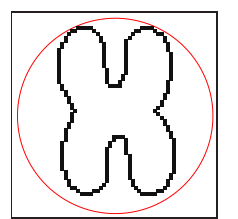
\includegraphics[width=5cm,height=4cm]{chapiter2/figures/FG01.png}
                \caption{initial contour}
        \end{subfigure}
        \hfill
        \begin{subfigure}[b]{0.3\textwidth}
                \centering
                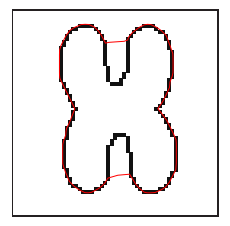
\includegraphics[width=5cm,height=4cm]{chapiter2/figures/FG02.png}
                \caption{Iteration 50}
        \end{subfigure}
        \hfill
        \begin{subfigure}[b]{0.3\textwidth}
                \centering
                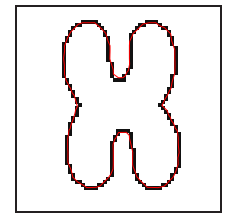
\includegraphics[width=5cm,height=4cm]{chapiter2/figures/FG03.png}
                \caption{GVF snake result}
        \end{subfigure}
        \caption{the convergence of the snake}
        \label{fig:figure5}
\end{figure}

\hspace{-0.6cm}The GVF field has a much larger capture range then the traditional snake,the GVF vectors are
pointing somewhat downward into the top of the U-shape, which
should cause an active contour to move farther into this concave as it's shown in figure(\ref{fig:figure6}) \cite{2.8}.\\
%sssss
\begin{figure}[ht!]
        \centering
        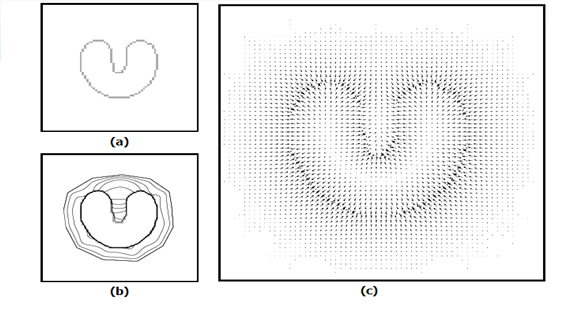
\includegraphics[width=10cm]{chapiter2/figures/FIG6.png}
        \caption{A snake with GVF external forces moves into the concave boundary region.}
        \label{fig:figure6}
\end{figure}

\begin{figure}[ht!]
        \centering
        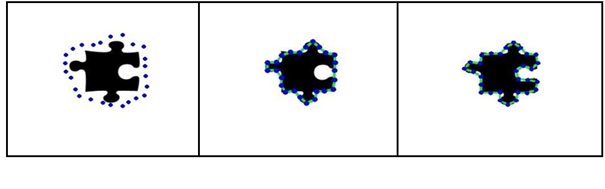
\includegraphics[width=15cm,height=4cm]{chapiter2/figures/FIG7.png}
        \caption{comparison between Traditional Snake and GVF Snake in concave shape}
        \label{fig:figure7}
\end{figure}
%ssssss
\hspace{-0.6cm}The application of the GVF snake model shows that the snakes can move into boundary concavities figure(\ref{fig:figure7})
as compared to the traditional snake model which cannot move in it.

\begin{figure}[ht!]
        \centering
        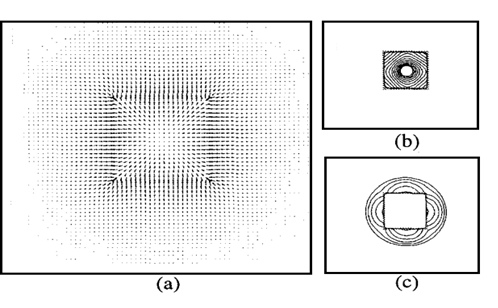
\includegraphics[width=10cm]{chapiter2/figures/FIG8.png}
        \caption{A GVF snake converges to the same result from either the inside or the outside \cite{2.8}}
        \label{fig:figure8}
\end{figure}

\begin{figure}[ht!]
        \centering
        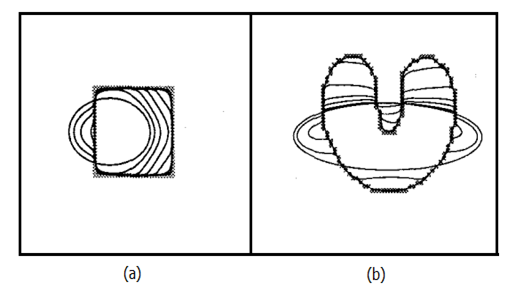
\includegraphics[width=15cm]{chapiter2/figures/FIG9.png}
        \caption{A GVF snake can also be initialized across the object boundary\cite{2.8}}
        \label{fig:figure9}
\end{figure}

\hspace{-0.6cm}Figure(\ref{fig:figure8}(a)) shows the computed GVF for the line drawing square shown using gray lines
,which show GVF snake results using initializations from the inside and outside (Fig(\ref{fig:figure8}(b)),Figure(\ref{fig:figure8}(c))) .\\
Figure(\ref{fig:figure9}(a)) and (\ref{fig:figure9}(b)) demonstrate a further initialization insensitivity: the initial snake can cross the boundary
.The three final configurations are nearly indistinguishable from each other, indicating that the GVF snake can be
initialized either inside or outside or across the desired boundary \cite{2.8}.

%!--------!
\section{Conclusion}\label{sec:conclusion-ch2}
In this chapter we looked at the parametric active contours that
are curves capable of detecting object boundaries through an energy
minimization process , a lot of approach are proposed to solve problems of the
traditional snake(initialization and have difficulties progressing into boundary
concavities), we focus on the GVF field which we will use it in our approach .